\documentclass[10pt]{article}
\usepackage[margin=17mm]{geometry}
\usepackage{graphicx,booktabs,hyperref}
\usepackage[strings]{underscore}
\setlength{\parindent}{0pt}\setlength{\parskip}{5pt}
\begin{document}
\section*{Wide quartic core: order, arithmetic and encoding}

Native correctness audit, 2026-10-25. Source c41a03785; frozen binary SHA
prefix f5180b12e9fc. Inputs m=16,17,18, first qualifying instance from seed 1,
cofactor cap 16; source-pinned internal search, not a priced candidate census.
Each rung and independent replay has 12-GiB address-space and 900-second caps.
All six processes exit zero; the three replay outputs are byte-identical.

\begin{center}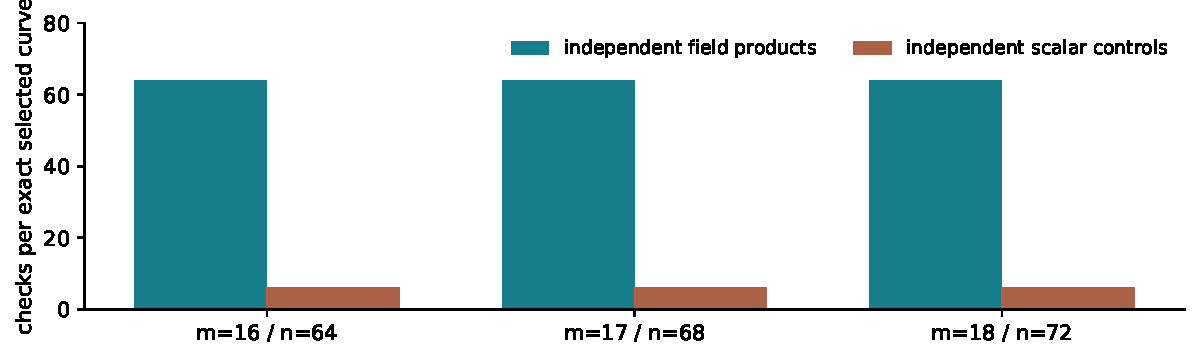
\includegraphics[width=\linewidth]{wide-controls.pdf}\end{center}
\begin{center}\small\begin{tabular}{rrrrr}\toprule
m & Seed & Full group order & Prime r & h\\\midrule
16 & 22 & 18446744076425775508 & 4611686019106443877 & 4 \\
17 & 14 & 295147905196116557432 & 36893488149514569679 & 8 \\
18 & 41 & 4722366482997941244794 & 2361183241498970622397 & 2 \\
\bottomrule\end{tabular}\end{center}
Each r is independently checked using BigUint modular exponentiation at the
first twelve prime Miller--Rabin bases, within the explicit deterministic
bound below $2^{73}$. A nonidentity on-curve G satisfies [r]G=O, independently
in polynomial-basis BinaryCurve arithmetic. Its unique multiple of r in the
exact Hasse interval certifies the full group order. Exact tower and
polynomial-basis coefficients, modulus and G are in each native JSON.

Addition, negation and six scalar controls agree with independent arithmetic;
scalars include $2^{65}+3$ and $2^{70}+2^{64}+123$. The first test point
has its highest field-coordinate bit set. Packing, decoding, full-width
decimal/hex strings and a planted four-point S5 relation are checked.
Old-rung field/point/scalar/native-count parity and exhaustive base-field
inversion/Artin--Schreier controls at m=16--18 pass in the library suite.
The full release library gate reports 4,634 passed, zero failed, 119 ignored;
the src/ tree remains identical to the frozen control revision c46089aed.

\textbf{Limits.} This is core correctness at L0 on the shared AMD EPYC
9V74 Linux x86-64 host. The legacy u64 CountedGroup/ecbench stage adapters
remain unintegrated. Full factor bases, oracle/relation collection, linear
algebra, complete DLP, matched rho and native physical prices at these sizes
are unmeasured. The original unsupported wider ecbench specs remain refusals.
No crossover or conclusion for prime-degree/prime fields follows.

\begin{flushleft}\footnotesize
Exact unregistered research-model ICV1 names:\par
\path{icv1-f2m64-tm2716223891-2b2a8430}\par
\path{icv1-f2m68-tm16763731575-8ae81c3a}\par
\path{icv1-f2m72-tm128296031097-38af8562}\par
Receipts: \path{../../pipeline-receipts/wide-core-audit-20261025/}\par
Full-suite metadata: \path{../../pipeline-receipts/wide-core-library-gate-20261025/}\par
Protocols: WIDE_CORE_PROTOCOL.md and WIDE_GROUP_AUDIT_PROTOCOL.md.
No additional paid VM was launched.
\end{flushleft}

\end{document}
